
\section{Instrumentation}

\textbf{Introduction}

Being both quantitative and experimental, physics is basically a science of measurement. A great deal of effort has been expended over the centuries improving the accuracy with which the fundamental quantities of length, mass, time, and charge can be measured.

It is important that the appropriate instrument be used when measuring. Ordinarily, a rough comparison with a numerical scale, taken at a glance and given in round numbers, is adequate. Increasing precision, though, requires a more accurate scale read to a fraction of its smallest division. The ``least count'' of an instrument is the smallest division that is marked on the scale. This is the smallest quantity that can be read directly without estimating fractions of a division.

Even at the limit of an instrument's precision, however, accidental errors--- which cannot be eliminated---still occur. These errors result in a distribution of results when a series of seemingly identical measurements are made. The best value, known as the most probable value, is the arithmetic mean or average of the measurements.

Other errors, characteristic of all instruments, are known as systematic errors. These can be minimized by improving the equipment and by taking precautions when using it.

\textbf{Length Measurement}

Three instruments will be available in this class for length measurements: \hspace{3pt} a ruler (one- or two-meter sticks, for example), the vernier caliper, and the micrometer caliper.

\textit{The Meter Stick}

A meter stick, by definition, is 1 meter (m) long. Its scaled is divided, and numbered, into 100 centimeters (cm). Each centimeter, in turn, is divided into 10 millimeters. Thus 1 cm = $10^{-2}$ m, and 1 mm = $10^{-1}$ cm = $10^{-3}$ m.

When measuring a length with a meter stick, different regions along the scale should be used for the series of measurements resulting in an average value. This way, non-uniformities resulting from the meter stick manufacturing process will tend to cancel out and so reduce systematic errors. The ends of the stick, too, should be avoided, because these may be worn down and not give a true reading. Another error which arises in the reading of the scale is introduced by the positioning of the eyes, an effect known as parallax. Uncertainty due to this effect can be reduced by arranging the scale on the stick as close to the object being measured as possible.

\textit{The Vernier Caliper}

A vernier is a small auxiliary scale that slides along the main scale. It allows more accurate estimates of fractional parts of the smallest division on the main scale.

On a vernier caliper, the main scale, divided into centimeters and millimeters, is engraved on the fixed part of the instrument. The vernier scale, engraved on the movable jaw, has ten divisions that cover the same spatial interval as nine divisions on the main scale:\hspace{4pt} each vernier division is $\frac{9}{10}$ the length of a main scale division. In the case of a vernier caliper, the vernier division length is 0.9 mm. [See figures below.]

\begin{center} \setlength{\unitlength}{1pt} \begin{picture}(330,125) \put(2,120){\makebox(0,0)[bl]{0}} \put(102,120){\makebox(0,0)[bl]{1}} \multiput(10,100)(10,0){12}{\line(0,1){10}} \multiput(9,96)(9,0){9}{\line(0,1){4}} \put(50,100){\line(0,1){15}} \put(45,93){\line(0,1){7}} \put(50,75){\makebox(0,0)[b]{0.00}}

\put(202,120){\makebox(0,0)[bl]{0}} \put(302,120){\makebox(0,0)[bl]{1}} \multiput(210,100)(10,0){12}{\line(0,1){10}} \multiput(214,96)(9,0){9}{\line(0,1){4}} \put(250,100){\line(0,1){15}} \put(250,93){\line(0,1){7}} \put(250,75){\makebox(0,0)[b]{0.05}}

\put(84,45){\makebox(0,0)[bl]{1}} \put(184,45){\makebox(0,0)[bl]{2}} \multiput(92,25)(10,0){13}{\line(0,1){10}} \multiput(114,21)(9,0){9}{\line(0,1){4}} \put(132,25){\line(0,1){15}} \put(150,18){\line(0,1){7}} \put(150,0){\makebox(0,0)[b]{1.23}}

\put(150,-20){\makebox(0,0)[b]{Examples of vernier caliper readings}}

\thicklines \multiput(0,100)(100,0){2}{\line(0,1){20}} \multiput(0,90)(90,0){2}{\line(0,1){10}} \put(0,100){\line(1,0){130}}

\multiput(200,100)(100,0){2}{\line(0,1){20}} \multiput(205,90)(90,0){2}{\line(0,1){10}} \put(200,100){\line(1,0){130}}

\multiput(82,25)(100,0){2}{\line(0,1){20}} \multiput(105,15)(90,0){2}{\line(0,1){10}} \put(80,25){\line(1,0){150}}

\end{picture} \end{center} \medskip

To measure length with a vernier caliper, close the jaws on the object and read the main scale at the position indicated by the zero-line of the vernier. The fractional part of a main-scale division is obtained from the first vernier division to coincide with a main scale line. [See examples above.]

If the zero-lines of the main and vernier scales do not coincide when the jaws are closed, all measurements will be systematically shifted. The magnitude of this shift, called the zero reading or zero correction, should be noted and recorded, so that length measurements made with the vernier caliper can be corrected, thereby removing the systematic error.

\textit{The Micrometer Caliper}

A micrometer caliper is an instrument that allows direct readings to one hundredth of a millimeter and estimations to one thousandth of a millimeter or one millionth of a meter (and, hence, its name). It is essentially a carefully machined screw housed in a strong frame. To measure objects, place them between the end of the screw and the projecting end of the frame (the anvil). The screw is advanced or retracting by rotating a thimble on which is engraved a circular scale. The thimble thus moves along the barrel of the frame which contains the screw and on which is engraved a longitudinal scale divided in millimeters. The pitch of the screw is 0.5 mm, so that a complete revolution of the thimble moves the screw 0.5 mm. The scale on the thimble has 50 divisions, so that a turn of one division is $\frac{1}{50}$ of 0.5 mm, or 0.01 mm.

Advance the screw until the object is gripped gently. Do not force the screw. A micrometer caliper is a delicate instrument.

To read a micrometer caliper, note the position of the edge of the thimble along the longitudinal scale and the position of the axial line on the circular scale. The first scale gives the measurement to the nearest whole division; the second scale gives the fractional part. It takes two revolutions to advance one full millimeter, so note carefully whether you are on the first or second half of a millimeter. The result is the sum of the two scales. (See examples below).

\vspace{0.3cm}
{\centering 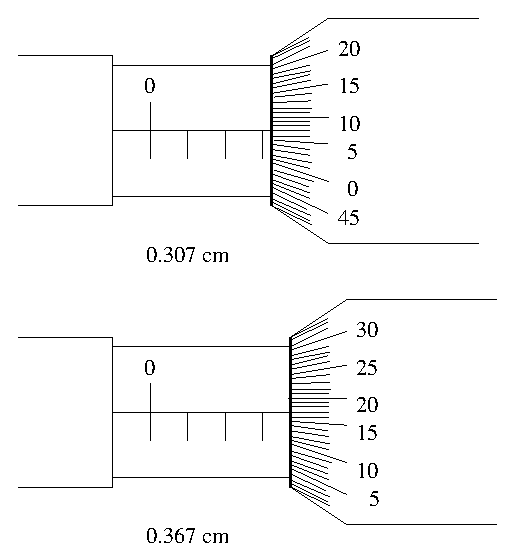
\includegraphics{appendices/instrumentation/instrumentation_fig1.eps} \par}
\vspace{0.3cm}

As with the vernier caliper, the zero reading may not be exactly zero. A zero error should be checked for and recorded, and measurements should be appropriately corrected.

\textbf{Mass Measurement}

Three kinds of instruments will be available to determine mass: a digital scale and two types of balances. The operation of the first instrument is trivial, and so will not be explained here.

Please understand that with each of these instruments we are really comparing weights, not masses, but the proportionality of weight and mass allows the instruments to be calibrated for mass.

\textit{The Equal-Arm Balance}

The equal-arm balance has two trays on opposite sides of a pivot. The total mass placed on one tray required to balance the object on the other gives the mass of the object. Most equal-arm balances have a slider, as well, that can move along a scale and allow for greater precision than the smallest calibrated mass available. Typically, this scale has 0.5 g divisions.

\textit{The Triple-Beam Balance}

The triple-beam balance, so-called because of its three slider scales, can be read to 0.1 g and estimated to half that. With an object on the tray, the masses of the different scales are slid to notches until balanced. Get close with the larger masses first and then fine-adjust with the smallest slider.

\textbf{Time Measurement}

Time measurements in this course will be made either with a computer or with a stop watch. This first is out of your control.

\textit{The Stop Watch}

The stop watches you will use in class have a time range of from hours to hundredths of a second. There are two buttons at the top: a stop/start button and a reset button. The operation of these should be evident, although once the watch is reset, the reset button also starts the watch (but doesn't stop it). Please be aware of this feature.

\textbf{Charge Measurements}

The magnitude of charge is among the most difficult measurements to make. Instead a number of indirect measurements are undertaken to understand electric phenomena. These measurements are most often carried out with a digital multimeter

\textit{The Digital Multimeter}

The digital multimeters available for laboratory exercises have pushbutton control to select five ac and dc voltage ranges, five ac and dc current ranges, and six resistance ranges. The ranges of accuracy are 100 microvolts to 1200 volts ac and dc, 100 nanoamperes to 1.999 amperes ac and dc, and 100 milliohms to 19.99 megaohms.

To perform a DC voltage measurement, select the DCV function and choose a range maximum from one of 200 millivolts or 2, 20, 200, or 1200 volts. Be sure the input connections used are V-$\Omega$ and COMMON. The same is true for AC voltage, regarding range and inputs, but the ACV function button should be selected.

For DC current choose DC MA (for DC milliamperes), while for AC current choose AC MA. Your choices for largest current are 200 microamperes or 2, 20, 200, or 2000 milliamperes. Check that the input are connected to MA and COMMON.

There are two choices for resistance measurement: Kilohms (K$\Omega$) and Megohms (20M$\Omega$). The input connectors are the same as when measuring voltage, namely V-$\Omega$ and COMMON. The range switches do not function with the Megohm function, but one of the range buttons must be set. The maximum settings for Kilohm readings are 200$\Omega$ or 2, 20, 200, or 2000k$\Omega$.

\newpage


\textbf{Calibrating Force Sensors}

1. Connect force sensor to Pasco interface (in port ``A'').

2. Open whatever software application you will be using in the current experiment.

3. Click ``Setup''.

4. Click ``Calibrate Sensors''.

FOR HORIZONTAL USE:

5. Set force sensor on track, and with no force applied to the sensor, press TARE button on side of the sensor. This sets the sensor to zero. Then set 1st calibration point to 0 newtons, press upper ``Read from sensor'' button.

6. While holding sensor stationary (with your hand), hang 200g from sensor over a pulley at end of track, as in Figure 2 of Experiment 13. Set 2nd calibration point to 1.96 newtons, press lower ``Read from sensor'' button.

7. Click ``OK''. Force sensor is now calibrated for the rest of your experiment. Close ``Calibrate Sensors'' window, close ``Setup'' window.

8. While still holding the force sensor still, press ``Start''. Graph should now show a reading of 1.96 N. Press ``Stop''.

9. Try hanging a different mass from the force sensor (over the pulley); press ``Start'' and check that it is reading correctly.

FOR VERTICAL USE:

5. Holding sensor vertically (with hook down and no force applied to it), press TARE button on side of the sensor. This sets the sensor to zero. Then set 1st calibration point to 0 newtons, press upper ``Read from sensor'' button.

6. Hang 200 g from sensor, set 2nd calibration point to 1.96 newtons, press lower ``Read from sensor'' button.

7. Click ``OK''. Force sensor is now calibrated for the rest of your experiment. Close ``Calibrate Sensors'' window, close ``Setup'' window.

8. While still holding the force sensor still, press ``Start''. Graph should now show a reading of 1.96 N. Press ``Stop''.

9. Try hanging a different mass from the force sensor; press ``Start'' and check that it is reading correctly.

